\chapter{Background}
This chapter presents a comprehensive theoretical overview of the key Artificial Neural Network used in this study: \textbf{Convolutional Neural Networks}. It also outlines the two main tasks covered in this document: \textbf{Instance Segmentation} and \textbf{Object Detection}. Finally, the chapter will provide an extensive review of performance metrics and visual explanations.

\section{Convolutional Neural Networks}
To recap our understanding from Feed Forward Networks, each neuron unit is represented and connected in a continuous chain-based architecture. Each layer is described by the following equation:
\begin{equation}
\boldsymbol{h}=f\left(\boldsymbol{W}\boldsymbol{x}+\boldsymbol{b}\right) \label{eq:ff:layer}
\end{equation}
where $\boldsymbol{h}$ denotes the output of the layer, $f$ is the activation function, $\boldsymbol{W}$ represents the weight vector, $\boldsymbol{b}$ is the bias vector, and $\boldsymbol{x}$ is the input vector of real values such that $\boldsymbol{x} \in \mathbb{R}^{n}$. In this formulation, the dimensionality $\mathbb{R}^{n}$ of $\boldsymbol{x}$ confines the input to a one-dimensional vector. Given this constraint, processing images in computer vision tasks using Feed Forward Networks leads to substantial computational complexity in matrix multiplication and results in vectors with high dimensionality of parameters.\\

Convolutional Neural Networks, as introduced by \textit{Kunihiko Fukushima}~\cite{Fukushima1980}, aim to address the challenge of dimensionality by utilizing a grid-like topology~\cite{Goodfellow-et-al-2016}. \textit{Le Cun et al.} further developed and elaborated on CNNs in their research~\cite{6795724, 726791}. They defined a Convolutional Neural Network based on three pivotal concepts: (I) local receptive fields, (II) shared weights, and (III) spatial or temporal subsampling~\cite{726791}.\\

\subsection{Local Receptive Fields}
As mentioned in the previous section, Feed Forward Networks consist of fully connected layers. The interaction is facilitated through connections between each neuron in the input layer and the corresponding neuron in the output layer, as illustrated in Figure \ref{fig:ff}. 
\begin{figure}[htb]
    \centering
    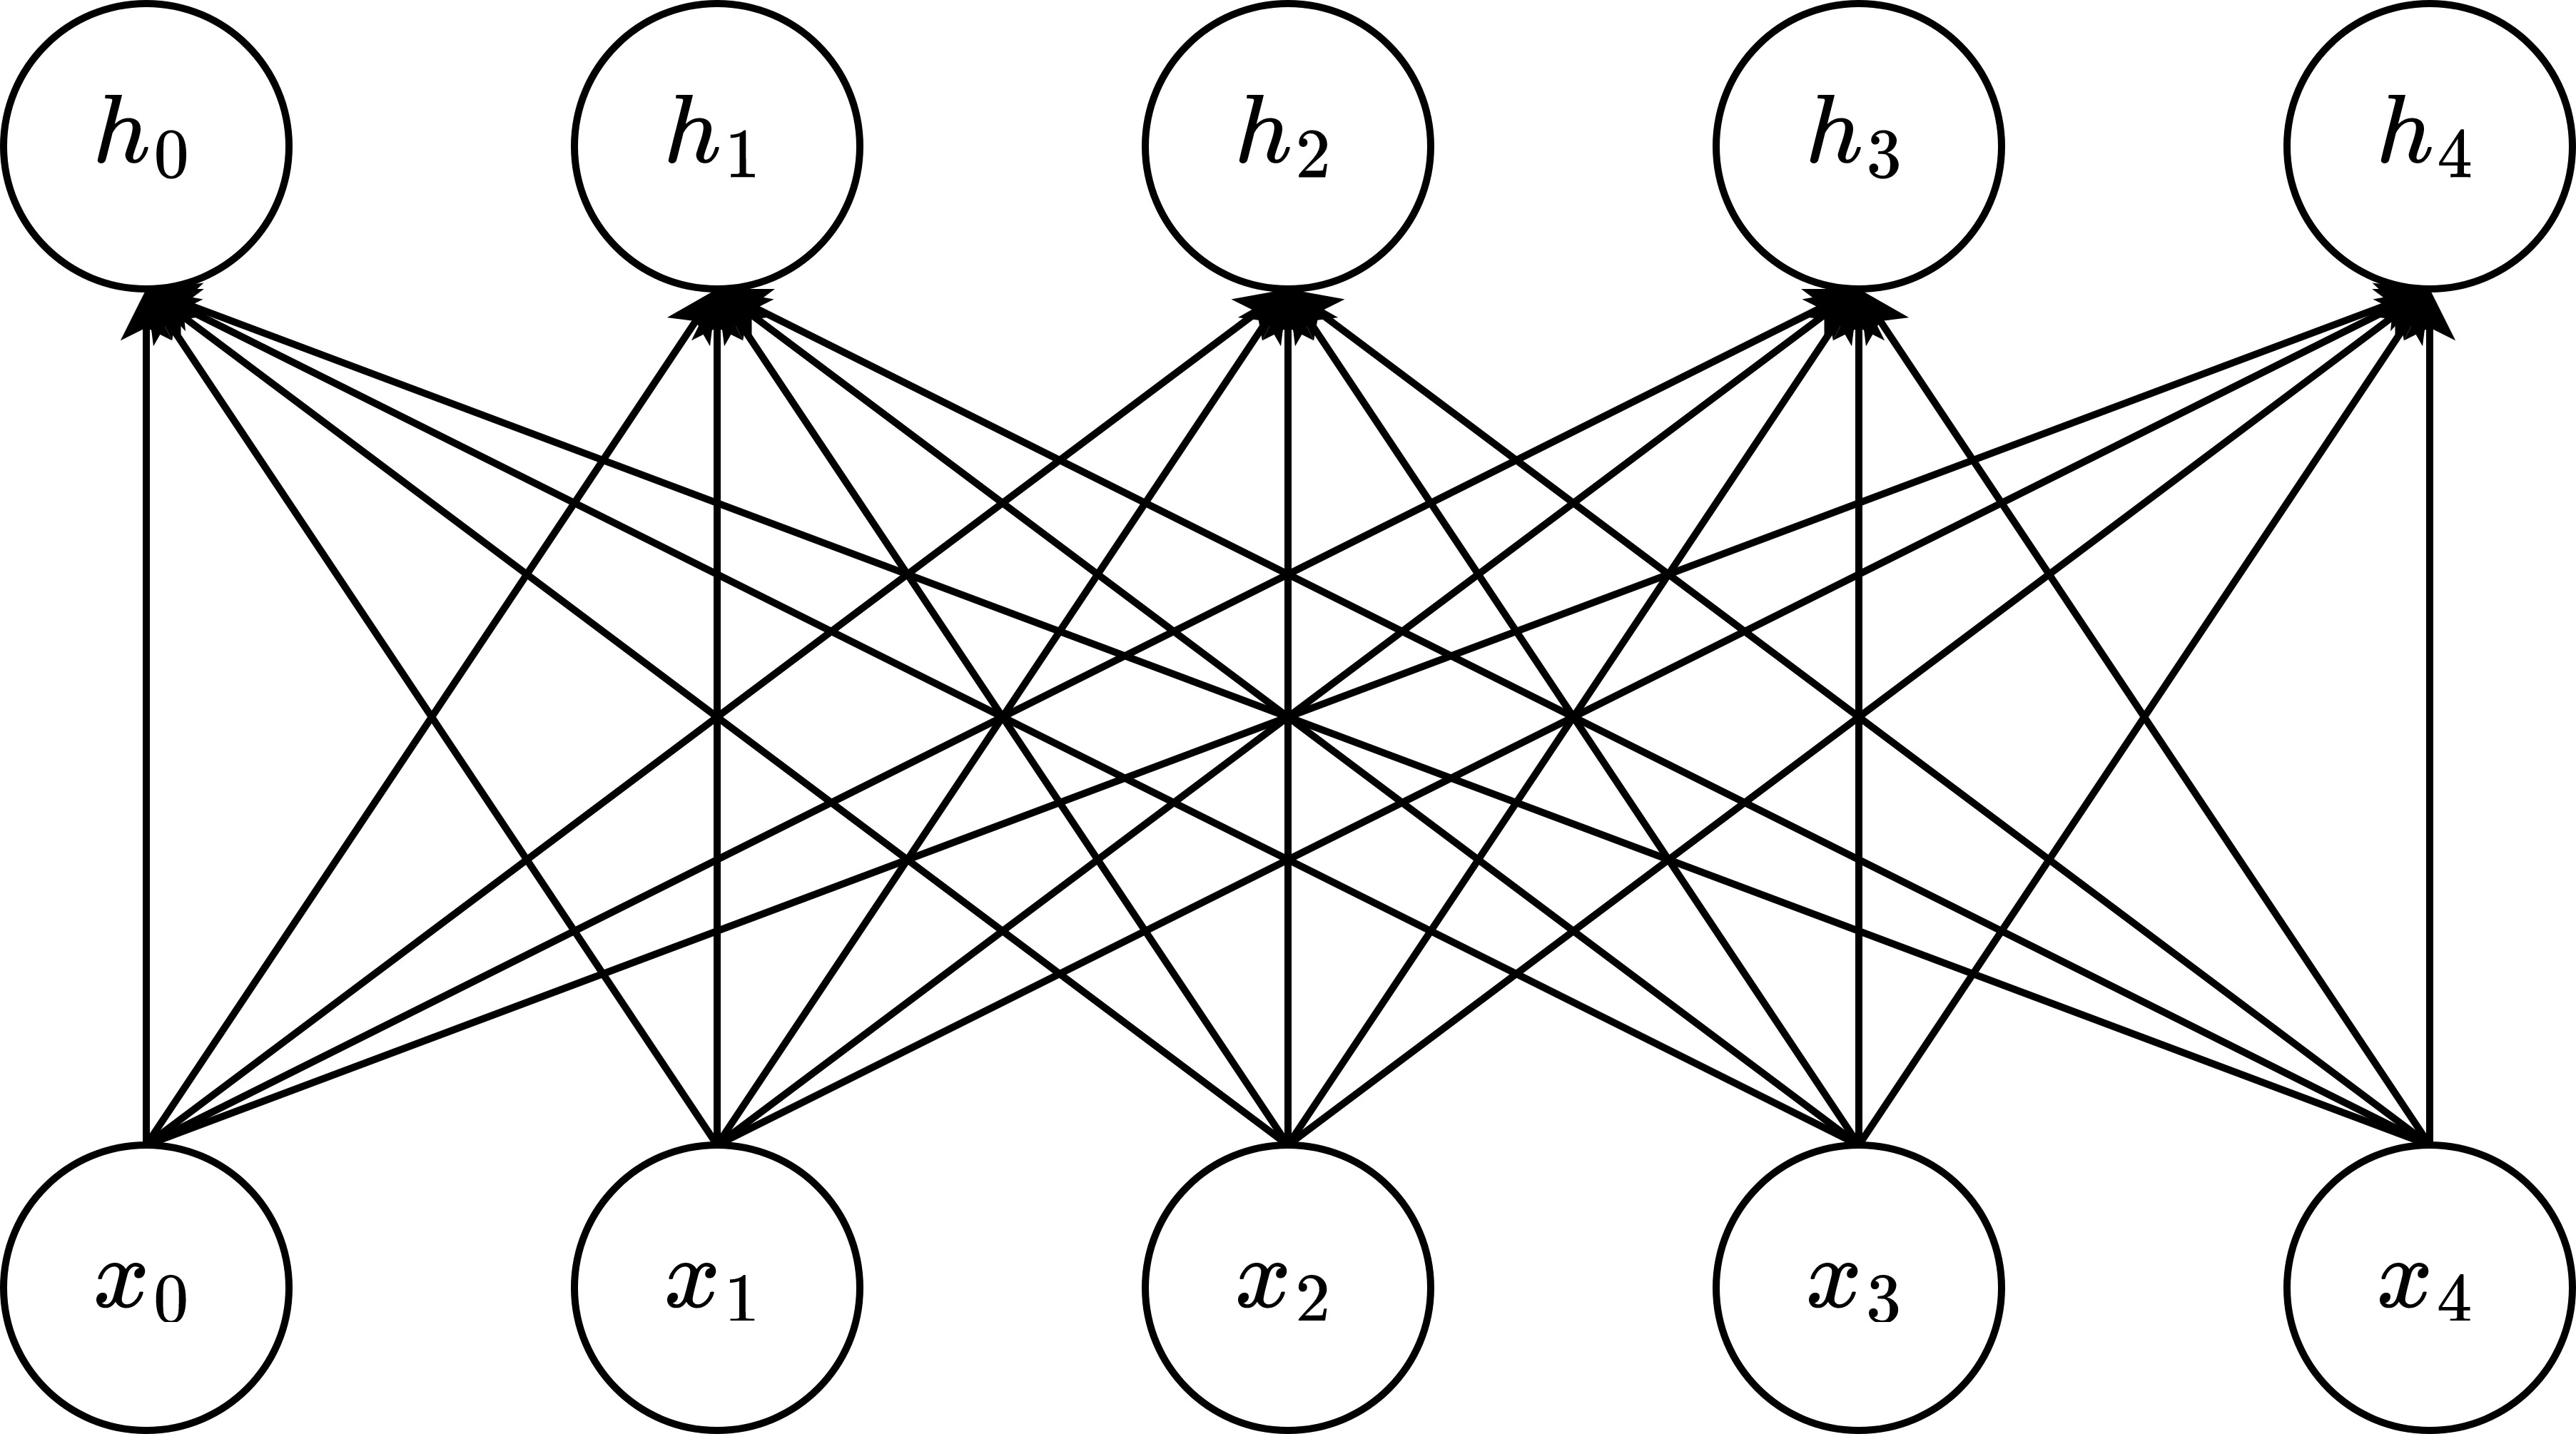
\includegraphics[width=0.5\linewidth]{figures/chapters-imgs/20/ff-net.jpg}
    \caption[Fully connected layer.]{Fully connected layer. Given an input $\boldsymbol{x} \in \mathbb{R}^{5}:\{x_{i}\in\boldsymbol{x},i=0,1,...,4\}$, the hidden layer $\boldsymbol{h}$ is defined following the equation (\ref{eq:ff:layer}).}
    \label{fig:ff}
\end{figure}

In CNNs, the connection is often restricted to a small neighborhood within the layer, as depicted in Figure \ref{fig:neighbourhood}. This limited neighborhood is termed the 'receptive field' and is employed in the convolution operation to compute sparse interactions in the input layer.
\begin{figure}[htb]
    \centering
    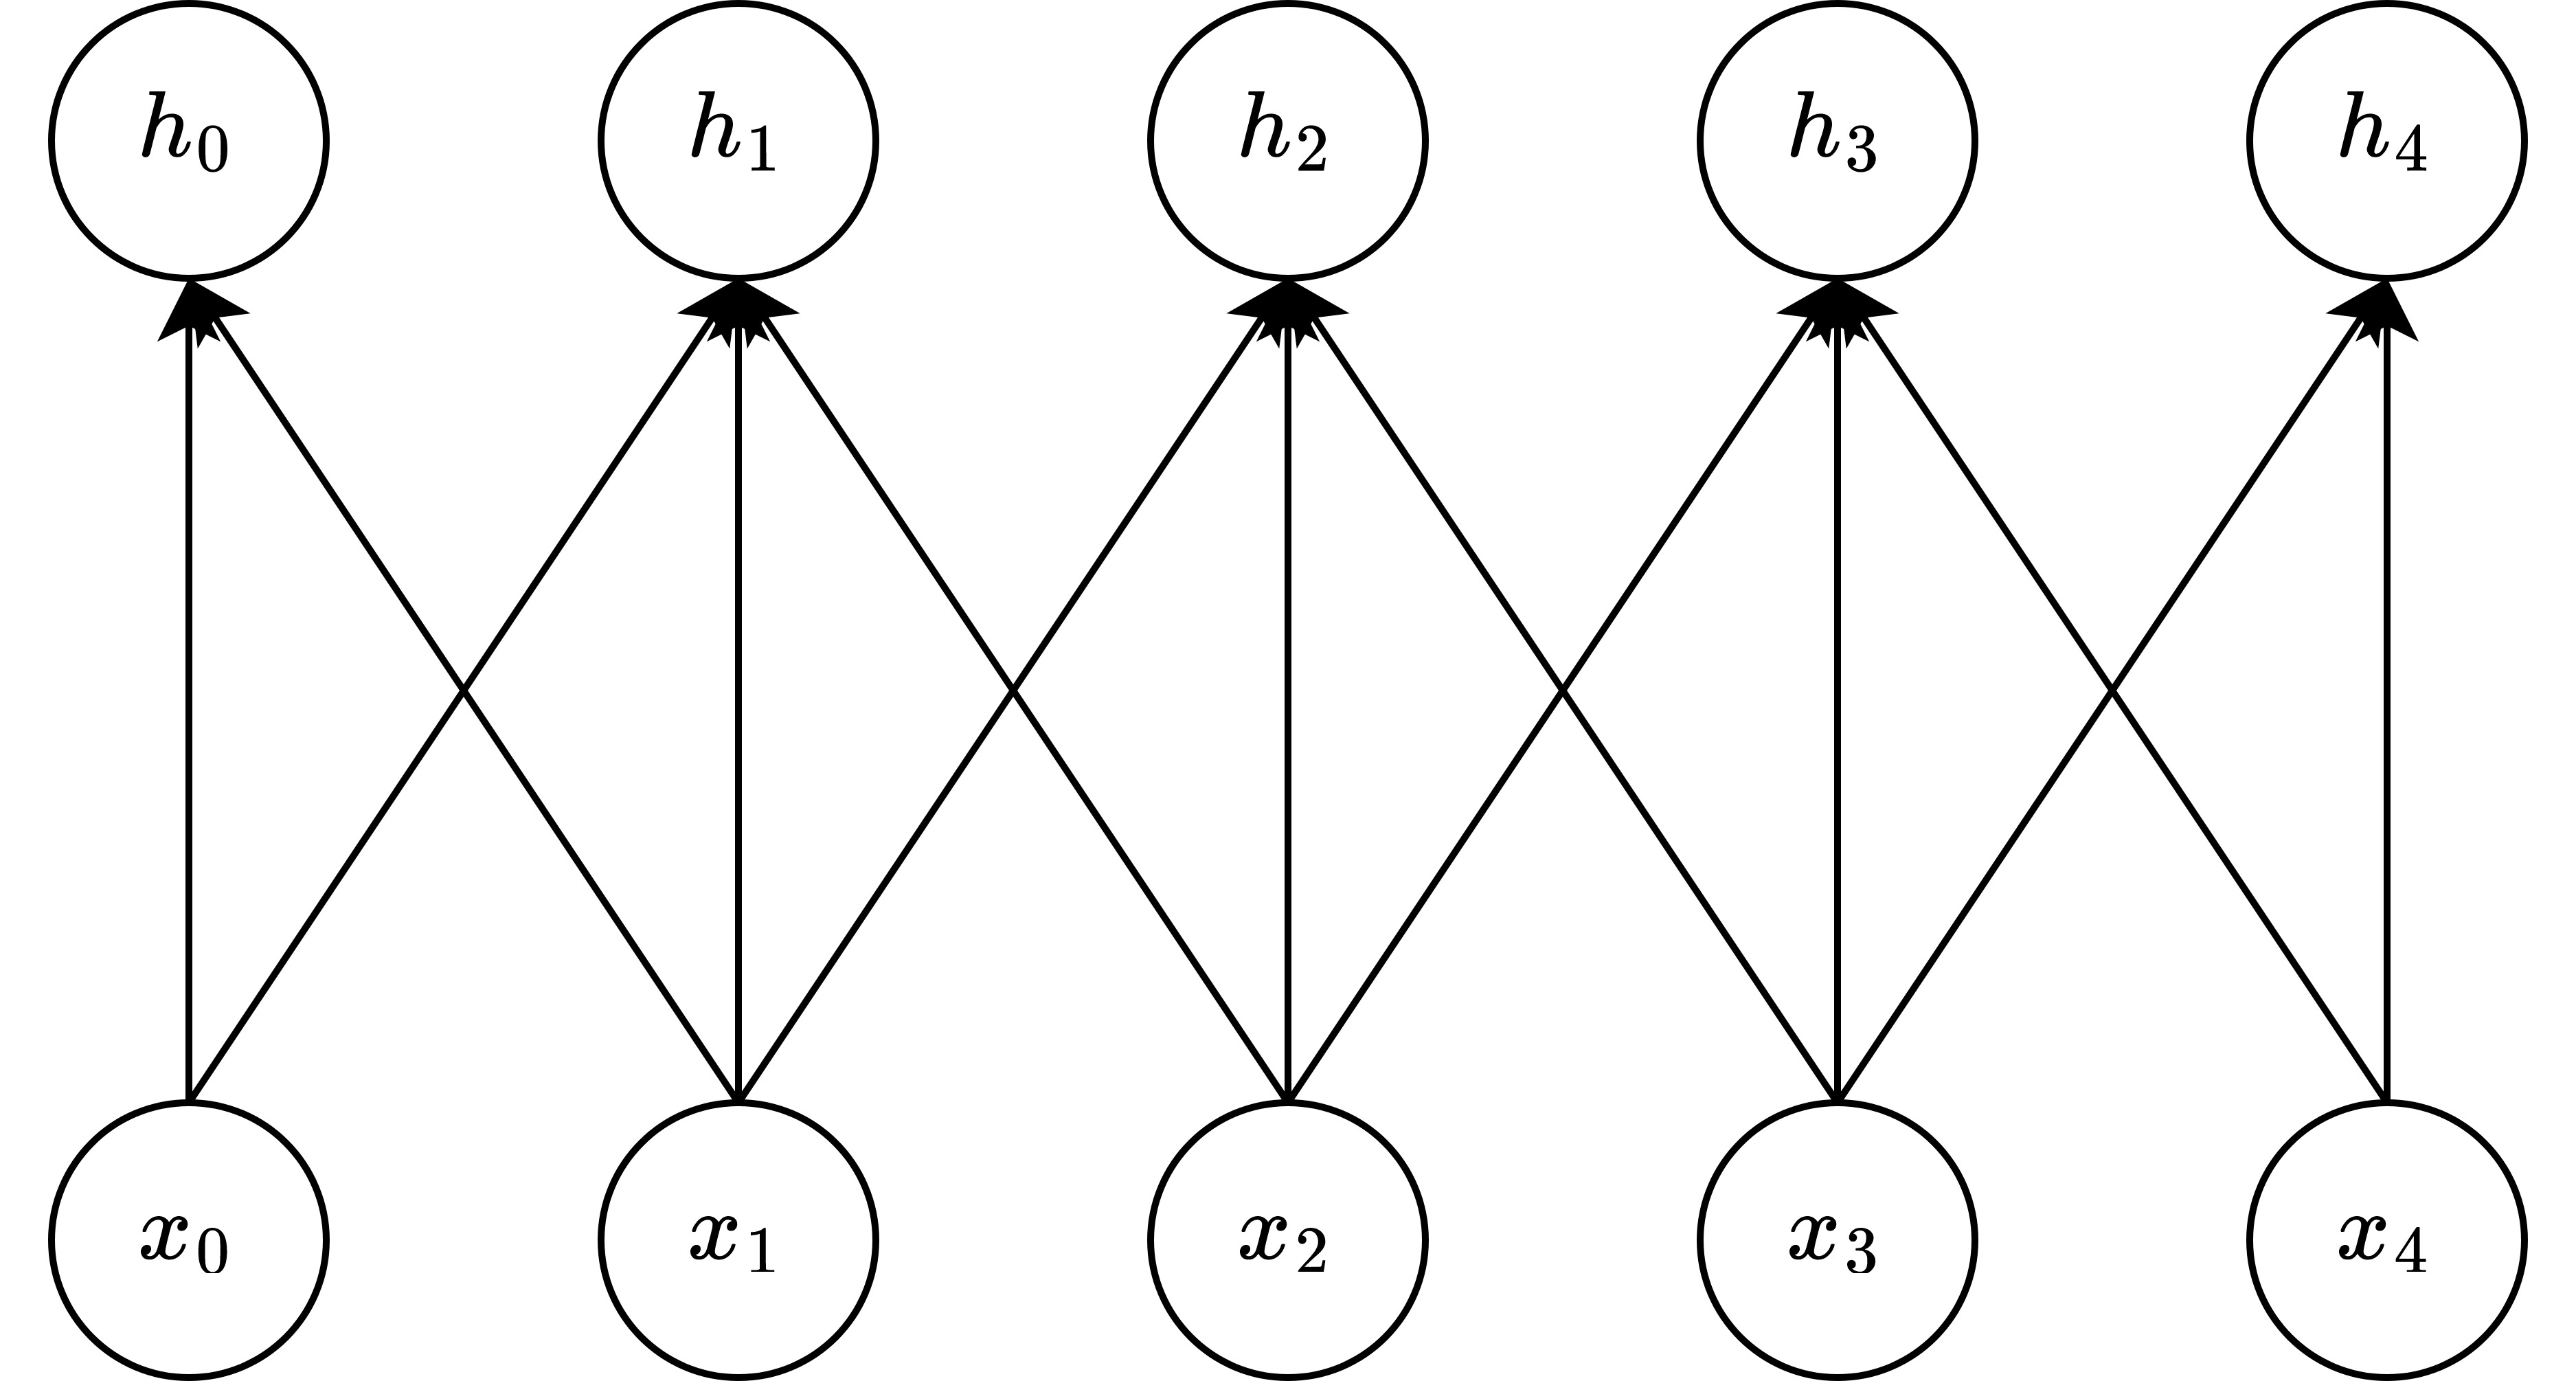
\includegraphics[width=0.5\linewidth]{figures/chapters-imgs/20/neighbourhood.jpg}
    \caption[Neighbourhood Convolutional Layer]{Convolutional Layer using neighborhoods: A variation of Figure \ref{fig:ff}}
    \label{fig:neighbourhood}
\end{figure}

The standard convolutional operation can be represented as:
\begin{equation*}
\boldsymbol{S}(t) = (\boldsymbol{x} * \boldsymbol{y})(t)
\end{equation*}
However, this function, being continuous in \(t\), is not directly applicable in a discrete setting. To address this, a discrete form of the convolution operation can be adopted~\cite{Arndt2011}:
\begin{equation}
\boldsymbol{S}[t]=\boldsymbol{x}[t] * \boldsymbol{y}[t]=\sum_{k=-\infty}^{\infty} \boldsymbol{x}[k] \cdot \boldsymbol{y}[n-k]. \label{eq:discrete:1d}
\end{equation}
Here, Equation (\ref{eq:discrete:1d}) alludes to a 1D convolutional operation, indicating that both \(\boldsymbol{x}\) and \(\boldsymbol{y}\) are 1D. For 2D operations~\cite{Arndt2011}, the equation takes the form:

\begin{equation}
\boldsymbol{S}[m, n]=\boldsymbol{x}[m, n] * \boldsymbol{y}[m, n]=\sum_{j=-\infty}^{\infty} \sum_{i=-\infty}^{\infty} \boldsymbol{x}[i, j] \cdot \boldsymbol{y}[m-i, n-j] \label{eq:discrete:2d}
\end{equation}
Equation (\ref{eq:discrete:2d}) correlates directly with the receptive field concept: in this context, \(\boldsymbol{x}\) represents the input, \(\boldsymbol{y}\) is the kernel, and \(\boldsymbol{S}\) denotes the feature map. Within this framework, connections remain localized within the 2D space of both the input vector and the kernel, as demonstrated in Figure \ref{fig:conv-op}.
\begin{figure}[htb]
    \centering
    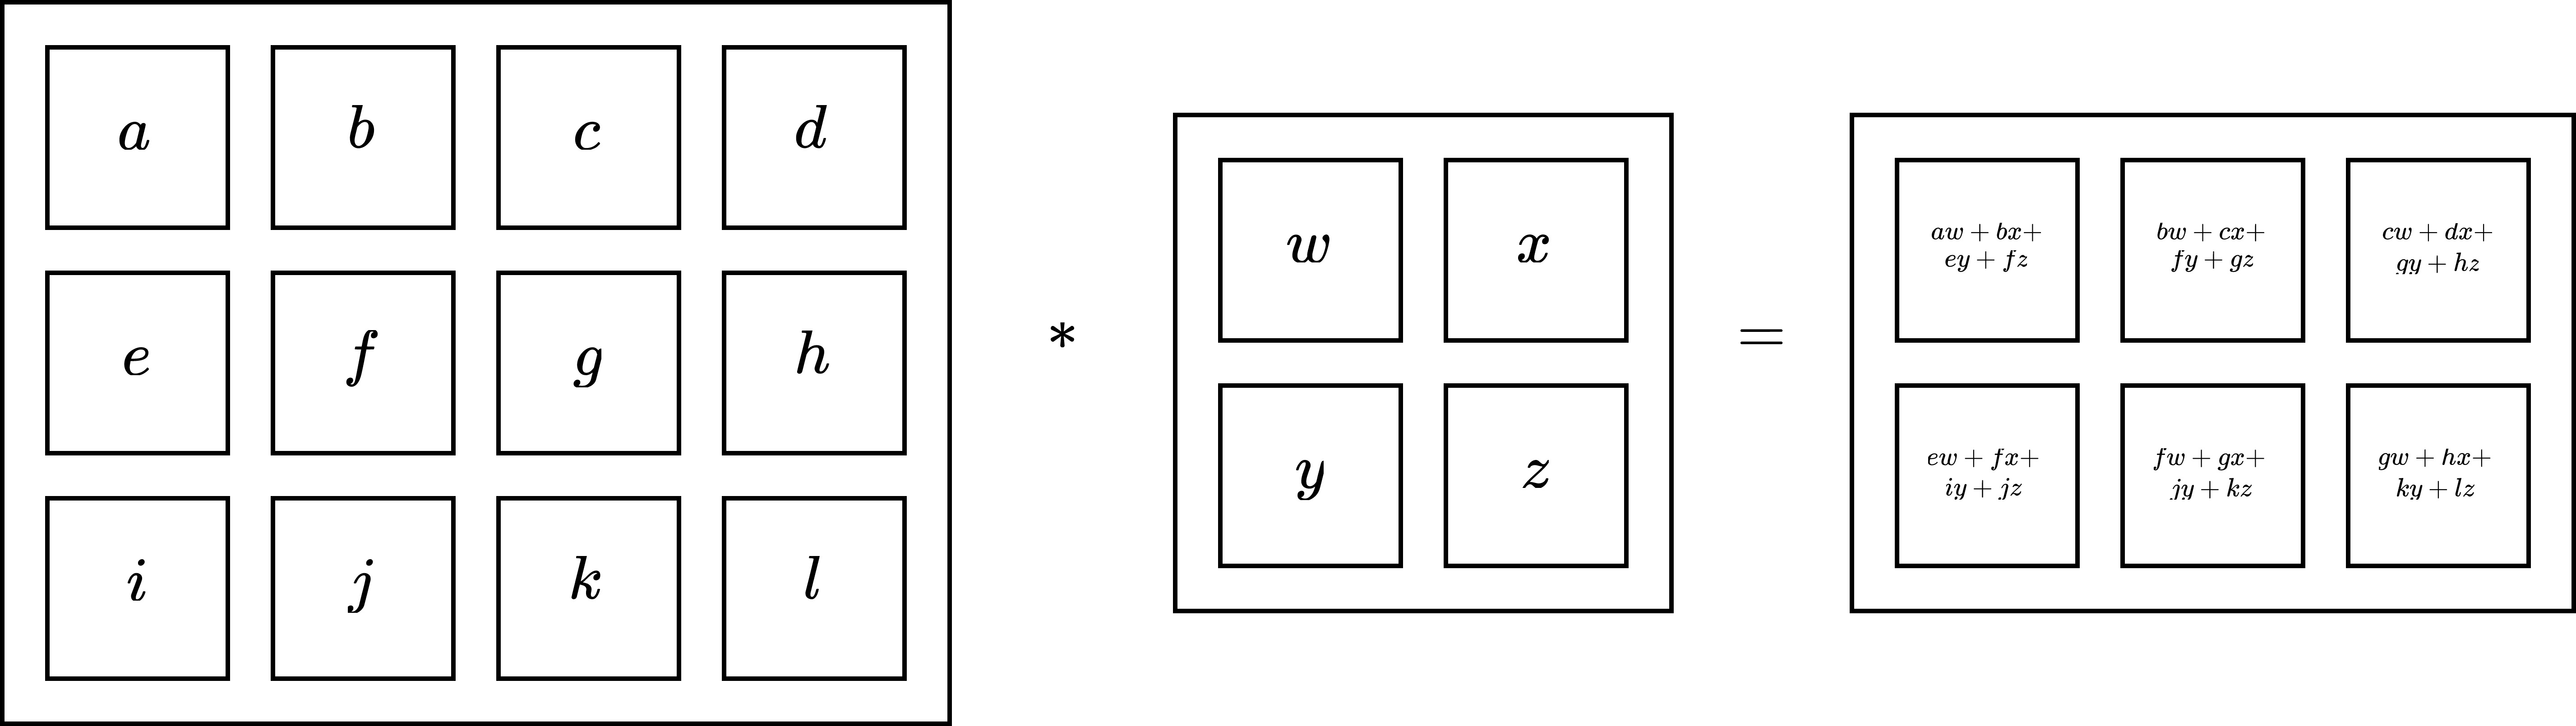
\includegraphics[width=0.9\linewidth]{figures/chapters-imgs/20/conv-op.jpg}
    \caption[Example of a convolutional operation involving an input \(\boldsymbol{x}\) and a kernel \(\boldsymbol{y}\).]{Example of a convolutional operation involving an input \(\boldsymbol{x}\) and a kernel \(\boldsymbol{y}\). Adapted image sourced from \cite{Goodfellow-et-al-2016}.}
    \label{fig:conv-op}
\end{figure}

\subsection{Shared Weights}
In CNNs, the convolutional layers use the equation (\ref{eq:discrete:2d}) to operate over the two dimension. In this process, the kernel $\boldsymbol{y}$ is shared for more than one function in a model~\cite{Goodfellow-et-al-2016}. This shared kernel is also know as the filter of the convolution that is convolved with the input. The Figure \ref{fig:conv-op}, display the a simple plane as input within which all the units share the same set of weights~\cite{726791}. An example of this can see in the Figure \ref{fig:no_padding_no_strides}.

\begin{figure}[htb]
    \centering
    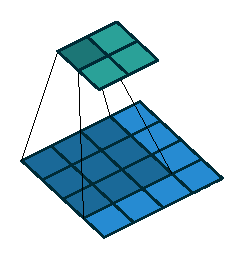
\includegraphics[width=0.24\textwidth]{pdf/no_padding_no_strides_00.pdf}
    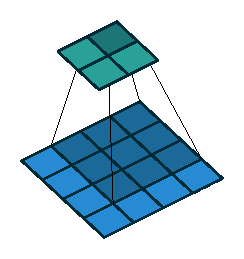
\includegraphics[width=0.24\textwidth]{pdf/no_padding_no_strides_01.pdf}
    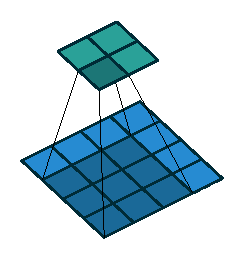
\includegraphics[width=0.24\textwidth]{pdf/no_padding_no_strides_02.pdf}
    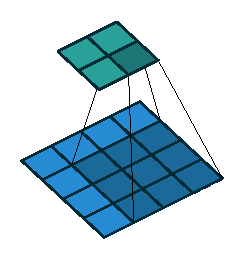
\includegraphics[width=0.24\textwidth]{pdf/no_padding_no_strides_03.pdf}
    \caption[Convolving a $3 \times 3$ kernel over a $4 \times 4$ input using unit strides.]{Convolving a $3 \times 3$ kernel over a $4 \times 4$ input using unit strides. Image and caption sourced from \cite{dumoulin2016guide}.}
    \label{fig:no_padding_no_strides}
\end{figure}

\subsubsection{Convolutional Layer}
Having defined the concepts of \textbf{Local Receptive Fields} and \textbf{Shared Weights}, we can express the convolutional layer in terms of equation (\ref{eq:ff:layer}) as:
\begin{equation}
\boldsymbol{h}=f\left(\boldsymbol{K}*\boldsymbol{x}+\boldsymbol{b}\right), \label{eq:conv:layer}
\end{equation}
where the operator \textbf{*} represents the convolution between the kernel vector \(\boldsymbol{K}\) (or the shared weights) and the input vector \(\boldsymbol{x}\).

\subsection{Spatial or Temporal Subsampling}
After applying the convolution operation, the positions of the values in the input vector become less relevant in the output vector or feature map. This can be problematic, especially as these positions may vary across different instances~\cite{726791}. This issue becomes even more pronounced when multiple convolutions are applied, as commonly occurs in layers. As a result, the extraction of distinctive features might shift in the location of the receptive field. One approach to address this problem is by reducing the precision with which the positions of distinctive features are encoded in a feature map. This reduction is akin to subsampling the output layer and is typically executed after one or more convolutional layers.

\subsubsection{Pooling Operation}
One operation used to reduce the feature map's dimensionality is the \textit{Pooling} operation, typically applied after one or more convolutional layers. This operation modifies the layer's output by summarizing its values. Consequently, the spatial dimension is reduced, yielding a new representation of the output with fewer parameters and computations.\\

The two most common pooling operations are:
\begin{itemize}
    \item \textit{Max Pooling}~\cite{Zhou1988ComputationOO}: This operation selects the maximum value from defined patches of a feature map.
    \item \textit{Average Pooling}~\cite{726791}: This operation computes the average value over specified patches of a feature map.
\end{itemize}
Both operations result in a downsampled version of the output feature vector, helping to produce a representation that remains relatively invariant to minor shifts in the input vector~\cite{Goodfellow-et-al-2016}.

\section{Computer Vision Tasks: Instance Segmentation and Object Detection}
\label{sect:comp-vision-tasks}
Convolutional Neural Networks have been instrumental in the realm of computer vision, initially applied to image classification tasks~\cite{6795724, 726791}. In these tasks, the network classifies images based on elementary visual features extracted, such as corners, edges, and endpoints. These features, processed across multiple layers of the network, are optimized to best represent the image in question. 

Emerging from this foundational task, the versatility of CNN-based approaches has expanded to encompass a broader spectrum of tasks like object detection, semantic segmentation, instance segmentation, object tracking, and more~\cite{Zou2023, Zaidi2022}. The purpose of this work focuses on two critical tasks: Object Detection and Instance Segmentation.

\subsection{Object Detection}
Object detection is an advancement of the primary task of image classification. While image classification identifies the main subject of the image, object detection aims to classify and recognize multiple objects within the image. These individual objects are referred to as \textit{instances}. The objective of object detection is to design a network that detects all of these instances annotated in an image. In this process, the network, also known as a \textit{detector}, must identify the position of each instance and then assign a coordinate \textit{bounding box} around it.\\

The foundation of the object detection task wasn't originally built upon the CNN architecture. It began with the pioneering work of \textit{Viola and Jones}~\cite{Viola2004, 990517}, who employed various techniques such as Haar-like features, integral images, Adaboost, and cascading classifiers~\cite{Zaidi2022}. Subsequently, \textit{Dalal and Triggs}~\cite{1467360} introduced the \textit{Histogram of Oriented Gradients~(HOG)} as a feature descriptor. Their detection approach utilized a grid-based decomposition of the image and created a gradient histogram for each grid element. These elements were then classified using a linear SVM.\\

However, prior models was based in the handcrafted features of the annotations. This problem was solved with the usage of the deep learning models, in more specific, the CNN models, due the ability to extract the high level features of the image. It's possible to identify two type of the CNN-based dectetor: \textbf{one-stage and two-stage detector}. In firs case, the two-stage detector, the model use a combination of backbone (in sometimes plus a neck) to extract the high level features and then pass it to a head that do the classify task. In the other hand, the one-stage network use an entire model to extract the feature and do the classify of the object in one pass-through stage.\\

In this work, we will focus on the two-stage model, which will be further described in Chapter \ref{chap:related-work}.

\subsection{Instance Segmentation}

Much like the previously discussed tasks of classification and object detection, image segmentation leverages the high-level features of an image to classify its pixels based on annotations. This overarching task can be further subdivided, with the most prominent and those explored in this work being semantic segmentation and instance segmentation~\cite{9356353, GU2022104401}. Semantic segmentation classifies each pixel of the image into object categories such as cars, people, or traffic signs. Conversely, instance segmentation delves deeper, identifying and segmenting pixels corresponding to individual instances present in the image, distinguishing between each person, each car, or each traffic sign.\\

The concept of instance segmentation was pioneered by \textit{Hariharan et al.} in their pioneer work titled \textit{Simultaneous Detection and Segmentation}~\cite{10.1007/978-3-319-10584-0_20}. Here, a two-stage network was utilized for both object detection and instance segmentation. Following this groundbreaking work, several state-of-the-art instance segmentation architectures emerged, utilizing the two-stage approach. One such architecture will be elaborated upon in Chapter \ref{chap:related-work}.

\section{Metrics and CNN Explanation}
To evaluated the performance of the models, it is necessary to summarise the principal metric commonly used for Object Detection and Instance Segmentation. On the other hand, in addition to performance metric of the models, we will define a strategy to evaluate the confidence of the proposal models and their respective variations, using visual and numerical evidence at the moment to compere these different models with each others.

\subsection{Metrics for Object Detection and Instance Segmentation} \label{sec:metrics}
Both Object Detection and Instance Segmentation metrics are based in the same metric reasoning: \textbf{where} and \textbf{what} a correct or incorrect area or object the model predicted. The most common way to measure the \textbf{where part}, is using the \textbf{Intersection over Union (IoU)}, or the \textbf{Jaccard Index}~\cite{Jaccard1912, 10.5169/SEALS-266450}, and is define as the measure of the area of intersection between the predicted segmentation mask $A$ (or the predicted bound box in the Object Detection) and the ground truth map $B$ (or the ground truth bound box in the Object Detection), divided by the area of the union between them, and is defined as:
\begin{equation}
\mathrm{IoU}=J(A, B)=\frac{||A \cap B||}{||A \cup B||},
\end{equation}
where $||\cdot||$ detonated the area of the set, and $J(A, B)$ the \textbf{Jaccard Index}, that is also in the range $0$ and $1$.\\

The most common way to measure the \textit{\textbf{what part}} a correct or incorrect area or object the model predicted from the beginning above definition, is using the classical terms \textit{True positive ($TP$), False positive ($FP$) and False negative ($FN$)}. Also, the \textit{True Negative (TN)} result are not used in the most command metrics, because indicate anywhere position where the model do not predict a mask or object and their respective annotation did not provide a mask or object; then the TN are vast and unnecessary to calculate. Whit this concepts, it is possible to define for each class, the \textbf{Precision} and \textbf{Recall} measure as:
\begin{align}
    \text { Precision }&=\frac{\mathrm{TP}}{\mathrm{TP}+\mathrm{FP}},\\
    \text { Recall }&=\frac{\mathrm{TP}}{\mathrm{TP}+\mathrm{FN}}.
\end{align}
Whit this two measure, it is possible to define the \textbf{Precision-Recall (PR) curve}, where it is show the relationship between Recall on the x-axis and Precision on the y-axis. In this case, the simple form to define a discrete definitions of this is using the \textbf{Intersection over Union} as a threshold for the points in the Precision-Recall (PR) curve:
\begin{equation}
    PR(A, B) = \sum^{|A|}_{i=0}\sum^{|B|}_{j=0}{PR(A_{i}, B_{j})\cdot I\left[ \mathrm{IoU}(A_{i}, B_{i})>\alpha \right]},
\end{equation}
where $|\cdot|$ detonated the length of the set, $PR(A_{i}, B_{j}$ represent the point of the Precision-Recall (PR) curve for each element of the set $A$ and $B$, $I\left[ \right]$ the indicator function, and $\alpha$ the $\mathrm{IoU}$ threshold. Then, it's possible to define the \textbf{mean Average Precision (AP)} as the area under the Precision-Recall (PR) curve for each $N$ classes as:
\begin{equation}
    \mathrm{mAP}=\frac{1}{N} \sum_{i=1}^{N} ||PR_{i}||.
\end{equation}

\subsection{CNN Model Explanation} \label{sec:explanation}
In the realm of designing and implementing Convolutional Neural Networks, deeper networks aim to achieve more complex representations of inputs compared to their shallower counterparts~\cite{Bengio2009}. Specifically, for tasks in image processing or computer vision, such intricate representations enable enhanced hierarchical depictions of images~\cite{DBLP:journals/corr/ZeilerF13}. This is attributable to how the multiple layers in the network effectively capture pertinent information. However, these deeper networks often present challenges in interpretability, as their predictions can be difficult to elucidate due to limited insight into their internal operations~\cite{Jung_2021_ICCV}.\\

To address this challenge, it is possible to employ advanced methods that offer improved interpretability and explanations of model performance. This facilitates a more robust evaluation when comparing different models. In this study, we aim to provide clearer insights into the behaviors of the proposed and tested models by utilizing a visual \textbf{\textit{class-discriminative location technique}} and a novel \textit{Remove and Debias} metric technique.

\subsubsection{Explanation model using Ablation CAM}
Visual explanations detailing how a model captures features across its layers can offer valuable insights into the model's internal behaviors. A novel avenue in this domain is the suite of \textbf{Class Activation Mapping (CAM)} based methods~\cite{DBLP:journals/corr/ZhouKLOT15, DBLP:journals/corr/SelvarajuDVCPB16, DBLP:journals/corr/abs-1710-11063, DBLP:journals/corr/abs-2008-02312, DBLP:journals/corr/abs-1910-01279, 9093360}. These techniques produce a \textbf{visual explanation map} by retaining spatial information throughout convolutional layers and underscoring the significance of each neuron for specific decision regions.\\

Drawing inspiration from the pioneering work of \textit{Bolei Zhou et al.}~\cite{DBLP:journals/corr/ZhouKLOT15}, the \textbf{visual explanation map}, given a model prediction \(f\) for a target class \(c\) of an input image \(x\), can be formulated as:
\begin{equation}
L_{\mathrm{CAM}}^c(A)=\operatorname{ReLU}\left(\sum_{k=1}^{N_l} w_{k}^{c} A_k\right), \label{eq:cam}
\end{equation}
where \(A = f^{[l]}(x)\) denotes the output of the \(l\)-th layer, \(A_k\) represents the \(k\)-th activation map of \(A\), and \(w_{k}^{c}\) is the \(k\)-th weight corresponding to class \(c\). The symbol \(N_l\) designates the count of activation maps in the \(l\)-th layer. Within the CAM paradigm, the coefficient \(w_{k}^{c}\) indicates the significance of \(A_k\)~\cite{DBLP:journals/corr/ZhouKLOT15}. Applying the \(\operatorname{ReLU}\) activation to the linear combination filters only the positive map values, thereby pinpointing pixels influencing the target class \(c\).\\

In this research, we adopt the approach described by \textit{Saurabh Desai et al.} in \textbf{Ablation CAM}~\cite{9093360}. This method is favored to avoid the gradient saturation issues faced by gradient-weighted strategies like \textit{Grad-CAM}~\cite{DBLP:journals/corr/SelvarajuDVCPB16}. Gradient saturation in these techniques leads to diminishing backpropagation gradients, consequently causing visualizations to falter in identifying pertinent image regions~\cite{9093360, DBLP:journals/corr/abs-2008-02312}.\\

Ablation CAM introduces a procedure wherein, for a given input image \(x\), a first forward pass through the model yields a non-linear function termed the \textbf{class activation score \(y^{c}\)} for class \(c\), derived from the activation map \(A_k\) of the final convolutional layer. In a subsequent forward pass with the same input image \(x\), individual activation cell values of the activation map \(A_k\) are set to zero. This leads to the ablation of the \(k\)-th unit, generating a new \textbf{class activation score \(y^{c}_{k}\)} to serve as a baseline for the activation map \(A_k\). The slope produced by this unit's ablation is defined as:
\begin{equation}
\text { slope }=\frac{y^c-y_k^c}{\left\|A_k\right\|}.
\end{equation}

Ablation CAM utilizes a modified version of this \textit{slope} to avoid small values that arise when the norm \(\|A_k\|\) is significantly larger than the difference \(y^c - y^c_k\). This modification defines the coefficient \(w_{k}^c\) in equation (\ref{eq:cam}) as:
\begin{equation}
w_k^c=\frac{y^c-y_k^c}{y^c},
\end{equation}
and this can be interpreted as the relative decrease in class activation score \(c\) upon the removal of activation map \(A_k\)~\cite{9093360}.

\subsubsection{Validate the explanation using imputation} \label{subsubsec:road}
A common method for validating explanation strategies is by perturbing the pixels of an image based on the importance assigned by these strategies. Specifically, the perturbation is determined by whether the pixel carries more or less critical information. Using this method, it is possible to measure the fidelity of the explanations~\cite{DBLP:journals/corr/abs-1912-01451}. This validation technique is often referred to as pixel-perturbation strategies, where a pixel is removed and replaced with an imputed value~\cite{DBLP:journals/corr/SamekBMBM15, DBLP:journals/corr/abs-1912-01451}. In our research, we employed a strategy named \textbf{ROAD (RemOve And Debias)} as proposed by \textit{Yao Rong et al.} in their study~\cite{DBLP:journals/corr/abs-2202-00449}.\\

The \textit{ROAD} strategy outlines two orders for pixel removal: \textbf{MoRF} (Most Relevant First) and \textbf{LeRF} (Least Relevant First)~\cite{DBLP:journals/corr/SamekBMBM15}. In the \textbf{MoRF} approach, the $k$ \textbf{most important features} of an instance are prioritized for removal. Given an explanation characterized by a choice of features through a binary mask, \(\boldsymbol{M} = \boldsymbol{e}_k(f, \boldsymbol{x}) \in\{0,1\}^d\), a value is set to one if the corresponding feature ranks within the top-$k$, and zero otherwise. The selection operator for the \textbf{least important dimensions}, denoted as \(\mathcal{M}_l:\{0,1\}^d \times \mathbb{R}^d \rightarrow \mathbb{R}^{d-k}\), extracts a vector, \(\boldsymbol{x}_l\), that retains only the remaining features, preserving their order based on their original input indices. The modified output of these features is expressed as \(\boldsymbol{x}_l^{\prime} = \mathcal{I}_l(\boldsymbol{M}, \boldsymbol{x}_l)\), where \(\mathcal{I}_l: \{0,1\}^d \times \mathbb{R}^{d-k} \rightarrow \mathbb{R}^d\) is an imputation operator. This operator repositions all inputs from \(\boldsymbol{x}_l\) to their original places, with the remaining set to a fill value, discarding the top-$k$ features. This procedure is illustrated in Figure \ref{fig:morf}. For the \textbf{LeRF} approach, the $k$ \textbf{least significant features} per instance are eliminated, with the selection operator defined for the \textbf{most important dimensions} as shown in Figure \ref{fig:lerf}.\\

The \textit{ROAD} strategy introduces an innovative imputation operator, \(\mathcal{I}_l\), termed \textbf{Noisy Linear Imputation}. This operator creates imputations that are not readily discernible, yielding a reduced \(I(\boldsymbol{x}_l^{\prime}; \boldsymbol{M})\). It approximates each pixel using a weighted mean of its neighbors, and a slight random noise is incorporated to ensure the model cannot easily learn the linear dependency.

\begin{figure}[htb]
    \centering % <-- added
\begin{subfigure}{0.45\textwidth}
  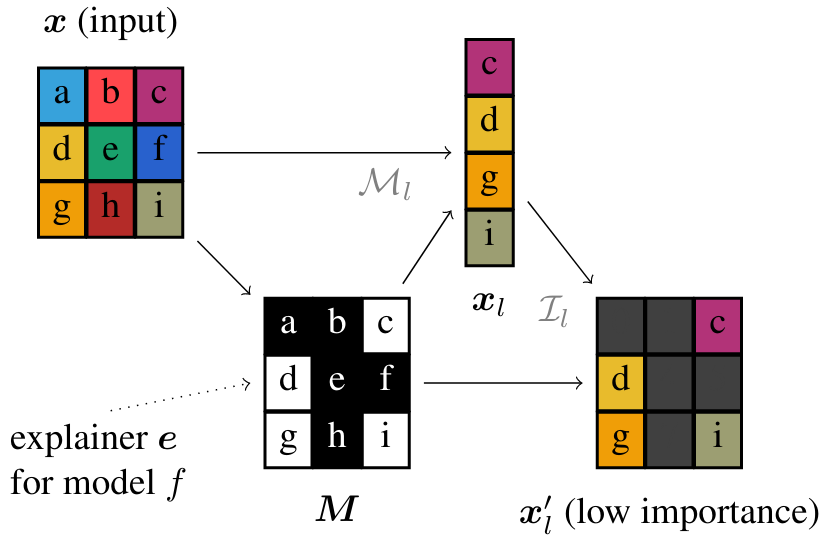
\includegraphics[width=\linewidth]{figures/chapters-imgs/20/morf.png}
  \caption{\protect\raggedright \textbf{MoRF} (Most Relevant First) order.}
  \label{fig:morf}
\end{subfigure} % <-- added
\medskip
\begin{subfigure}{0.45\textwidth}
  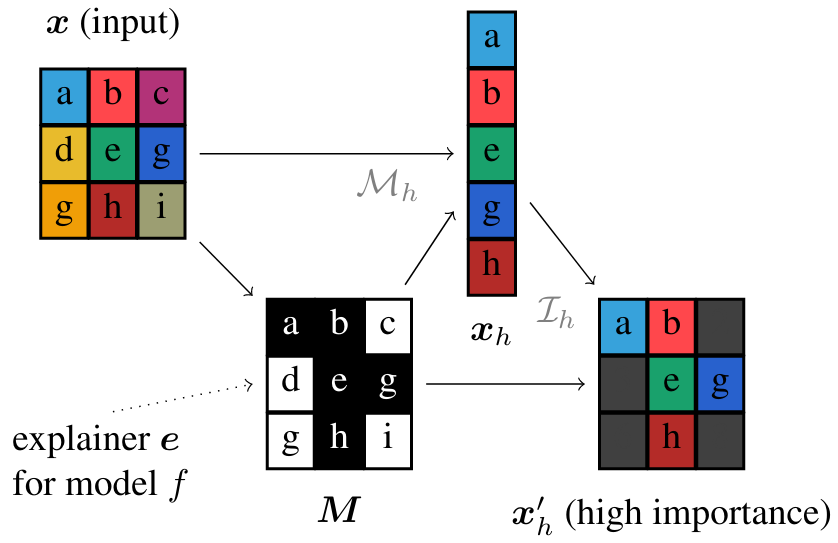
\includegraphics[width=\linewidth]{figures/chapters-imgs/20/lerf.png}
  \caption{\protect\raggedright \textbf{LeRF} (Least Relevant First) order.}
  \label{fig:lerf}
\end{subfigure}
\caption[\textbf{MoRF} (Most Relevant First) and \textbf{LeRF} (Least Relevant First) pixel removal sequences utilized by the \textbf{ROAD} approach]{\textbf{MoRF} (Most Relevant First) and \textbf{LeRF} (Least Relevant First) pixel removal sequences utilized by the \textbf{ROAD} approach. Images sourced from~\cite{DBLP:journals/corr/abs-2202-00449}.}
% \label{fig:}
\end{figure}